\chapter{Analysis \label{anal}}
This chapter introduces malware analysis (see~\autoref{anal:malware}) and differentiates the techniques (see~\autoref{anal:malware:dyn_stat}), outlines and describes mechanisms and environments utilized by cyber security professionals and companies (see~\autoref{anal:malware:mech_envs}), describes the virtualization technology KVM (see~\autoref{anal:virtual:kvm}) and the orchestration mechanism Kubernetes (see~\autoref{anal:k8s}).

\section{Malware analysis \label{anal:malware}}
Monitoring a malicious actor, sample or an entity in any environment is interchangeable from the analyst point of view. Therefore, knowing the malware analysis techniques is crucial for secure monitoring of malicious actors. Malware analysis may be static and dynamic with varying tools and mechanisms \cite{article:malware_analysis_techniques} \cite{research:malware_analysis_2017}.

\subsection{Dynamic and static \label{anal:malware:dyn_stat}}
Dynamic analysis is a process of actively monitoring, ideally in an isolated environment, the execution of a malware sample. Static analysis, as the name implies, inspects the function calls, readable strings, control and data flow of a malware sample (i.e. binary, program code).

% DYNAMIC ANALYSIS LIMITATIONS:
Dynamic analysis may be unsafe and devastating, unless environment or system isolation is applied, but it's more precise and bypasses the reversing of self-modified code. Even though, dynamic analysis does not explore all execution paths, there are techniques resolving this drawback (i.e. virtual machine snapshots \cite{research:malware_analysis_2017}). Additionally, dynamic analysis in an isolated or virtualization environment is exposed to the risk of isolation detection \cite{medium_article:malware_analysis_sandboxing}, meaning the executed malicious program stops or even self-destructs.

%STATIC ANALYSIS LIMITATIONS:
Static analysis is safe [and inspects all execution paths of the binary], but may be difficult to interpret when malicious actors utilize the obfuscation, compression or encryption techniques. Advanced malware sample poses a challenge for a malware analyst due the usage of control-flow flattening \cite{report:eset_static_analysis} and other methods. It suggests that dynamic malware analysis bypasses this troublesome procedure and discloses the sample outcome or agenda.

Manual Egele, et al. in their article \cite{article:malware_analysis_techniques} highlight the problems of static malware analysis approaches. The authors introduce multiple state-of-the-art techniques and tools dedicated to dynamic malware analysis - Function Call Monitoring, Function Parameter Analysis focusing of the final values, Information Flow Tracking, Instruction Trace and Auto start Extensibility Points (monitor startup programs, cron jobs, etc.).
% TODO: consider more detailed explanation of the techniques

\subsection{Bait and execution environments \label{anal:malware:mech_envs}}
These mechanisms must provide solution to dynamic malware analysis limitations in order to effectively capture the malicious actor's agenda. It should be a robust system implying the impression of a production environment.

\subsubsection*{Honeypot and honeynet \label{anal:malware:mech_envs:hons}}
Honeypot is a bait service, system or a even whole network (honeynet) usually hosted on public server. Its main purpose is to be scanned, attacked or compromised by the malicious actor. Every honeypot provides the desired functionality of the target resource, to mimic the production environment, leaving the malicious actor unaware of the honeypot \cite{study:enisa_honeypots}.

Based on the ENISA honeypot study \cite{study:enisa_honeypots}, honeypots are classified from the level of interaction view and based on the attacked resource type. The Low Interaction Honeypot (LIH) provides very low availability of the host OS. Most services and application are mocked and simulated in a static environment. Everything accessible is controlled by a decoy application with absolutely minimal in-depth features (e.g. shell, configuration files, other programs etc.). LIHs are more secure for the host, but far less capable or useful for malware/attack detection and inspection.

On the contrary, High Interaction Honeypot (HIH) is a fully responsive system with live applications and services with minimal to none emulated functionalities. It provides the attacker a wide attack surface ranking the HIH far less secure with the whole OS at the malicious actor's disposal. The idea is to make HIHs believable as possible and isolating it from production environment including virtualization \cite{blog:first_malware_analysis}.

Honeypots are differentiated by the type of attacked resource. The server-side honeypot is the well-known honeypot with running service(s) and monitoring the activity of the server-side connections. The attacked resources are the services listening on the dedicated ports. It's main purpose is to detect and identify botnets and forced authentication/authorization attempts.

The client-side honeypot is deployed as a user application, which utilizes the server's services. The monitored subject is the application (e.g web-browser, document editor). It's main purpose is to detect client-side attacks originating from the application (i.e. web-browser attacks via web pages and plugins).

% TODO: maybe briefly define honeypot classifications in the footnotes and define honeypots technically in-depth

\subsubsection*{Sandbox \label{anal:malware:mech_envs:sand}}
In the security branch, sandbox is used for controlled both static and dynamic malware analysis as mentioned in \autoref{anal:malware:dyn_stat}. It is dedicated for execution or testing of unverified functionality, behavior of programs or other activity \cite{article:fortinet:sandbox}. Moreover, the environments hosting or serving as a sandbox must be isolated to secure any spreading. A possible attack of this kind is referred to as the escape attack, which is a vulnerability allowing a malicious actor to move from virtualized/containerized environment to the host system.

"When a threat is contained within the sandbox environment, it is quarantined and available for study by the in-house IT team or external cybersecurity experts" \cite{article:fortinet:sandbox}. Slightly changing the notion makes a sandbox technology ideal for active and live analysis of malicious actors. Other benefits are flexibility of easily changing the environment to adapt to the current scenario.

\section{Virtualization technology \label{anal:virtual}}
The section discusses thesis related virtualization technologies kernel virtual machines (KVM), Docker containerization and the Kubernetes orchestration mechanism. Together these technologies may create a sandboxed honeynet holding theoretically multiple environments, thanks to the Kubernetes capabilities.

\subsection{Kernel-based Virtual Machine \label{anal:virtual:kvm}}
% TODO: why KVM and libvirt. KVM is a type-1 (bare-metal) hypervisor technology which enables VMs to exist in the host system. libvirt is the API daemon for VM configuration and specification
KVM is a type-1 (bare-metal) hypervisor enabling technology used for virtualization of full operating systems. The core functionality is based on the kernel capabilities to manage the hardware resource, hence the name "Kernel-based" VM \cite{redhat:kvm}. KVM is native to the Linux as a kernel module, which requires the host machine processor virtualization support and by utilizing them, multiple VMs may coexist on one machine \cite{article:kvm_qemu}.

\subsubsection*{KVM, QEMU and Libvirt \label{anal:virtual:kvm:combined}}

Although, KVM is not a complete solution without the \textit{libvirt} virtualization API daemon and the \textit{QEMU} hardware emulation \cite{docs:qemu}. When referring to KVM, it is often substituted for both KVM and QEMU. The combination provides a performance considered nearly native-like \cite{article:kvm_qemu}. While the KVM kernel module translates code in the kernel-space, QEMU provides the virtualization and emulation of hardware resources. In addition, Libvirt is a virtualization management tool and API. It is fully configurable by automation mechanism to automate the whole process of VM creation.

Libvirt is the solution to the variations of virtual machine images, since each technology has a different format. For example the storage backend provides the same API of so called volumes for any image format \cite{docs:libvirt:volume}. Apart from all of the libvirt objects available, networking is the most relevant. According to the API specification \cite{docs:libvirt:network}, the configuration options are for both VM network and host interface with DHCP, DNS and NAT. Additionally, there is also support for \textit{openvswitpch}, which is particularly useful for more complex network architectures with VLANs and other protocols and standards.

Nevertheless, libvirt and thereby KVM/QEMU is compatible with the Linux bridge \cite{docs:libvirt:network}, which is a simple virtual network component used for connecting networks \cite{docs:arch:bridge}. Creation and maintenance is straightforward and the functionality is effective enough to connect the VMs with the host machine. An advantage is it can be managed by various control tools (e.g. \textit{ip command}, \textit{ifupdown}, \textit{bridge-utils} and other), which provides the separation of the development environment setup and the main host environment.

\subsubsection*{Vagrant \label{anal:virtual:kvm:vagrant}}
According to official documentation\cite{docs:vagrant}, Vagrant is a VM provisioning technology and one level up in terms of KVM virtualization. Meaning, it adds another configuration layer for a whole multi-VM environment. It composes of manifest file called Vagrantfile. This file is a ruby program using specific calls to defined and configure multiple VMs. Vagrant is ideal for completely bypassing the direct usage of Libvirt and instead utilize the Vagrant libvirt provider\footnote{Open-source solution to the vagrant libvirt provider - \url{https://github.com/vagrant-libvirt/vagrant-libvirt}}. In a Kubernetes blog \cite{blog:k8s:vagrant}, the author describes multi-node Kubernetes cluster deployment using Vagrant with Ansible. It is practical approach to deploy a custom base environment with additional configuration using third-party tools e.g. Ansible.

% TODO: mention vagrant and mainly vagrant boxes and configuration possibilities i.e. vagrant-libvirt, networking, ruby language for configration freedom because it's not bound to configration variables but the full language syntax is available for creating numerous varying VMs

\lstinputlisting[language=Ruby, style=custom, caption={Working Vagrantfile example with the 'generic/ubuntu1804' using the libvirt provider and configuring 2GB or RAM, 2 virtual CPUs, DHCP network interface, libvirt storage pool to 'default'.}, label=listing:vagrantfileexample]{assets/listings/Vagrantfile.example}

%Vagrantfile
The fact that Vagrantfile is a ruby program provides the freedom of not being bound to a set of configuration variables and other related limitations. The definition is enclosed in \texttt{Vagrant.configure()} call and further divided in to \texttt{config.vm}, \texttt{config.ssh} and \texttt{config.vagrant} sections. \texttt{config.vm} is the context for configuring the VM directly with Vagrant e.g. vagrant box, provider, networking, disk. \texttt{config.ssh} is for configuring SSH access for the vagrant utility and \texttt{config.vagrant} is used for modifying Vagrant itself like plugins.

The API is unified across all Vagrant providers and is enriched by provider-specific variables as the \texttt{libvirt\_\_network\_address} on line 19 in \autoref{listing:vagrantfileexample}. With the capabilities of \textit{vagrant-libvirt} provider, the VM can be defined is this one file - Vagrantfile.

% vagrant boxes
Another term is the Vagrant box. It is a specifically formatted unit packaging the VM image, which is ready for deployment. A box can found in public repositories e.g. Vagrant Cloud\footnote{\url{https://app.vagrantup.com/boxes/search}} similarly to the Docker Hub. Benefit is the customization and direct workflow when creating a box, because then it can be reused for other VMs are share the same configuration and setup.

\subsection{Docker \label{anal:virtual:docker}}
% TODO: switch order with Kubernetes to maintain postupnost virtualizacie
% only short mainly about that video which covers it all
% container spying through mergeddir and other things
% searching for processes running in container etc.
Docker is very popular containerization technology used by developers and in production environments. Therefore a detailed explanation is not in scope of this thesis. On other hand this section covers deeper aspects of Docker and its mostly containers.

Similarly to Vagrant (see~\autoref{anal:virtual:kvm:vagrant}), a Docker image is defined in a manifest file called Dockerfile. The image is used to create a Docker container as a single unit. Multiple containers can share an image with different configuration to adapt to the current environment e.g. database configuration, port publishing, storage mounting. 

But, each container is uniquely identified by an ID and other resources and objects belonging to the single container e.g. mapped network interface, storage volumes. When not specifically configured, both networking and volumes/storage would be local to the container and be removed along with the container. In either case the data, networking and yet unmentioned processes are accessible from the host system. Main reference for the base information is the \texttt{docker inspect} command, which returns every settings, mounted directory, networking configuration and execution metadata.

Julia Evans constructively discusses various container spying techniques dedicated to Docker in a video demonstration \cite{video:docker:spying}. Apart from Docker-specific spying with the \texttt{inspect} command, there is \texttt{nsenter} and the inspection of \texttt{overlayfs}. Nsenter is nearly equivalent to the \texttt{docker exec} command, but it executes a command with a specified namespace \cite{man:nsenter}. Despite knowing the container namespace, it has no requirements and is Linux native. The advantage over \texttt{docker exec} is that for nsenter the executed command/program (see~\autoref{listing:nsenter:example}) does not needs to be installed in the target container.

\lstinputlisting[language=bash, style=codestyle, caption={Executes the \texttt{ip address} command within the network (option \texttt{-n}) namespace of a taget process with ID 6234}, label=listing:nsenter:example]{assets/listings/nsenter_cmd.example}

"OverlayFS is a modern union filesystem that is similar to AUFS, but faster and with a simpler implementation" \cite{docs:docker:overlayfs}. As the Docker image is build, each compact change creates a new layer of the container root file system linked to the previous layer and including the difference. These layers can be inspected in the host system as bare directories. Mounted volumes are no exception and both can be identified from the \texttt{docker inspect} command output. \textit{/var/lib/docker/overlay2} stores all these layers (see~\autoref{listing:overlay2:example}). 

\lstinputlisting[language=bash, style=custom, caption={Container files, independent of the layer, are accessible from the host system. For example output the contents of an arbitrary file}, label=listing:overlay2:example]{assets/listings/overlay2.example}

Useful information in the \texttt{docker inspect} output:
\begin{itemize}[noitemsep]
	\item Main process ID.
	\item Path to the top layer of the overlay file system.
	\item List of mounted volumes and directories.
	\item Network interface.
	\item Environment variables.
\end{itemize}

\section{Kubernetes \label{anal:k8s}}
This section covers the Kubernetes concepts focusing on the aspects essential for properly organizing an efficient setup. That includes Kubernetes nodes, Pods, Deployments, Services and persistent storage resources. \textit{Disclaimer: the following concept definitions are derived from the official Kubernetes documentation page} \cite{docs:k8s:concepts}.

\subsection{Components and nodes \label{anal:k8s:nodes}}
Kubernetes is a platform for orchestrating multiple containers among its cluster nodes. A functional cluster comprises of control-plane components i.e. API server, \textit{etcd}, Pod scheduler, controller manager and cloud-specific controller manager. The \textit{kubelet}\footnote{Communicates with the API server on the master node. Ensures that the Pods are up and running}, \textit{kube-proxy}\footnote{The node networking endpoint for Pod communications.} and container runtime components run on every node, wheres the control-plane components aside on a single node - control-plane node\footnote{Also referred to as the master node. The current Kubernetes documentation does not mention this node role anymore.}. All other nodes are called workers.

When creating or updating a cluster, nodes are registered in the API server by kubelet or manually. A node must be considered healthy to run a Pod, which si important because the environment/cluster may be highly dependent on the node's computational resources. The declarative nature of Kubernetes simplifies the creation of development environments. The configuration defines a desired state of an application ecosystem, microservices or other custom environment and the control-plane schedules and assign the Pods to suitable nodes \cite{video:k8s:principals}. 

\subsection{Resources \label{anal:k8s:resources}}
\begin{figure}[h]
	\centering
	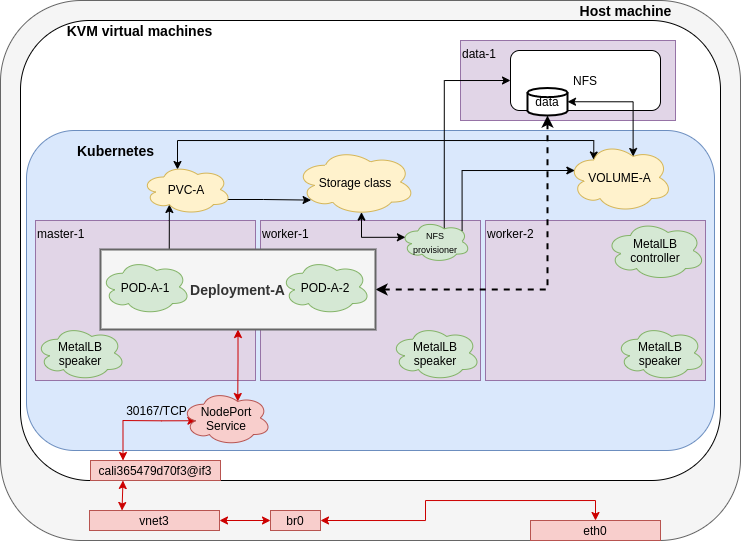
\includegraphics[scale=0.6]{k8s_arch}
	\caption{Kubernetes sample architecture with Pods, Deployments, Services and Volumes. A 'cloud' is a Kubernetes component (green = Pod, yellow = volume-related objects, red = Service and network-related objects). Lines represent communication links and the dotted lines are abstract/logical connections.}
	\label{image:anal:k8s:arch}
\end{figure}

Kubernetes environments are build upon API resources or objects.

\subsubsection*{Workloads \label{anal:k8s:resources:workloads}}
Mainly the smallest running unit - Pod encapsulates one or more containers, storage resource and a unique network identifier. Best is to run single application instance per Pod \cite{docs:k8s:concepts:pods}. Above is a ReplicaSet\footnote{Definition of horizotally scaled Pods with a specific number of replicas.} and Deployment, which at first glance fulfills the same, except that Deployment (see the Deployment object in \autoref{image:anal:k8s:arch}) is a abstraction above Pods and ReplicaSets combined. Kubernetes suggests that "you may never need to manipulate ReplicaSet objects: use a Deployment instead" \cite{docs:k8s:concepts:replicasets}. Deployments allow rolling updates of both ReplicaSets and Pods. In comparison to \textit{docker-compose}, the definition of the container(s) in the Deployment resource is very syntactically similar.

\subsubsection*{Volumes \label{anal:k8s:resources:volumes}}
Kubernetes, dy default, does not provide data persistence, as it is in docker by design. There are various options of mounting volumes to Pods via PersistentVolumes (PV) e.g. cloud-specific volume plugins or \textit{hostPath}. The PV is linked to a special resource PersistentVolumeClaim (PVC), which is manually created alongside a Pod and binds to a suitable PV object \cite{docs:k8s:concepts:persistentvolumes}. In other words, PVC is a request for assigning a PV to Pod/Deployment. Although the PV must be created and meant all requirements of the PVC in case of successful binding. For that reason a PV template called StorageClass exists, which dynamically creates PVs for subsequent binding (refer to \autoref{image:anal:k8s:arch} for graphical representation of the relations).

Since for this thesis the Kubernetes cluster is local and bare-metal (no cloud and in VMs) and hostPath expects the Pod(s) to remain on the same node\footnote{This can be resolved by using Taints and schedule the Pod only on the specified node. Although this beats the purpose of Kubernetes} \cite{docs:k8s:concepts:volumes}. The Network File System (NFS) is supported on any Linux system (as a NFS server) and has Kubernetes provisioner integration \cite{git:nfs}.

\subsubsection*{Service \label{anal:k8s:resources:service}}
By default every Pod running a network service is unable to communicate with the outside network or other applications within the cluster, except for the shared containers in the same Pod. The Service resource cooperates with the kube-proxy component, which assigns the Service a virtual IP address (also called ClusterIP) visible only inside the cluster \cite{docs:k8s:concepts:service}.

The level of access via the Service depends on its type - ClusterIP, NodePort, LoadBalancer and ExternalName. To open a Service to the outside network (see the red section in \autoref{image:anal:k8s:arch}) any type but ClusterIP serves this purpose. The ExternalName requires a functional kube-dns component and NodePort does not map the service port to a reserved port, but instead uses a port from immutable range (30000-32767) \cite{docs:k8s:concepts:service}.

A LoadBalancer is a cloud provider-specific Service type combining NodePort and Cluster in a way to expose the Service over a public IP address. An advantage is an existing bare-metal implementation\footnote{MetalLB - Metal Load Balancer is a bare-metal LB implementation utilizing either a RM-OSI layer 2 routing or BGP \cite{docs:metallb}.} and the ability to expose reserved ports (e.g. 22, 80, 443).

\section{Environment monitoring \label{anal:mon}}
Knowing what and how to extract and monitor is vital to understanding the threat actor's agenda. There are various mechanisms and possibilities to effectively observe container activity events i.e. file system, networking and process execution. Full related solutions are documented in the next chapter (see~\autoref{related}). Regarding the expected setup of virtual machines hosting the Kubernetes cluster, the possible monitoring strategies are:

\begin{itemize}[noitemsep]
	\item From within the container as an agent reporting events over an associated Service.
	\item Abuse the container-host mapped resources (e.g. network interfaces, container mounted directories) and stealthily spying.
\end{itemize}

Container monitoring from the container itself may appear more straightforward, but it's similar to monitoring of a honeypot, where agents could be discovered or in other way uncovered by the threat actor. Since containers are wrapped environments hosted on the host machine, the file system, networking processes are readable. The apparent advantage is a transparent view of any monitoring for the threat actor, since the container has an enclosed environment by namespaces \cite{blog:containers}. For example docker with the \textit{overlay} file system driver has a predefined location where each container root FS exists (unless the volume binding overrides this).

\subsection{Existing tools \label{anal:mon:exist}}
This section outlines a briefly discusses various applicable and suitable container activity monitoring tools.

\subsubsection*{BPF Compiler Collection (BCC)}
\begin{figure}[h]
	\centering
	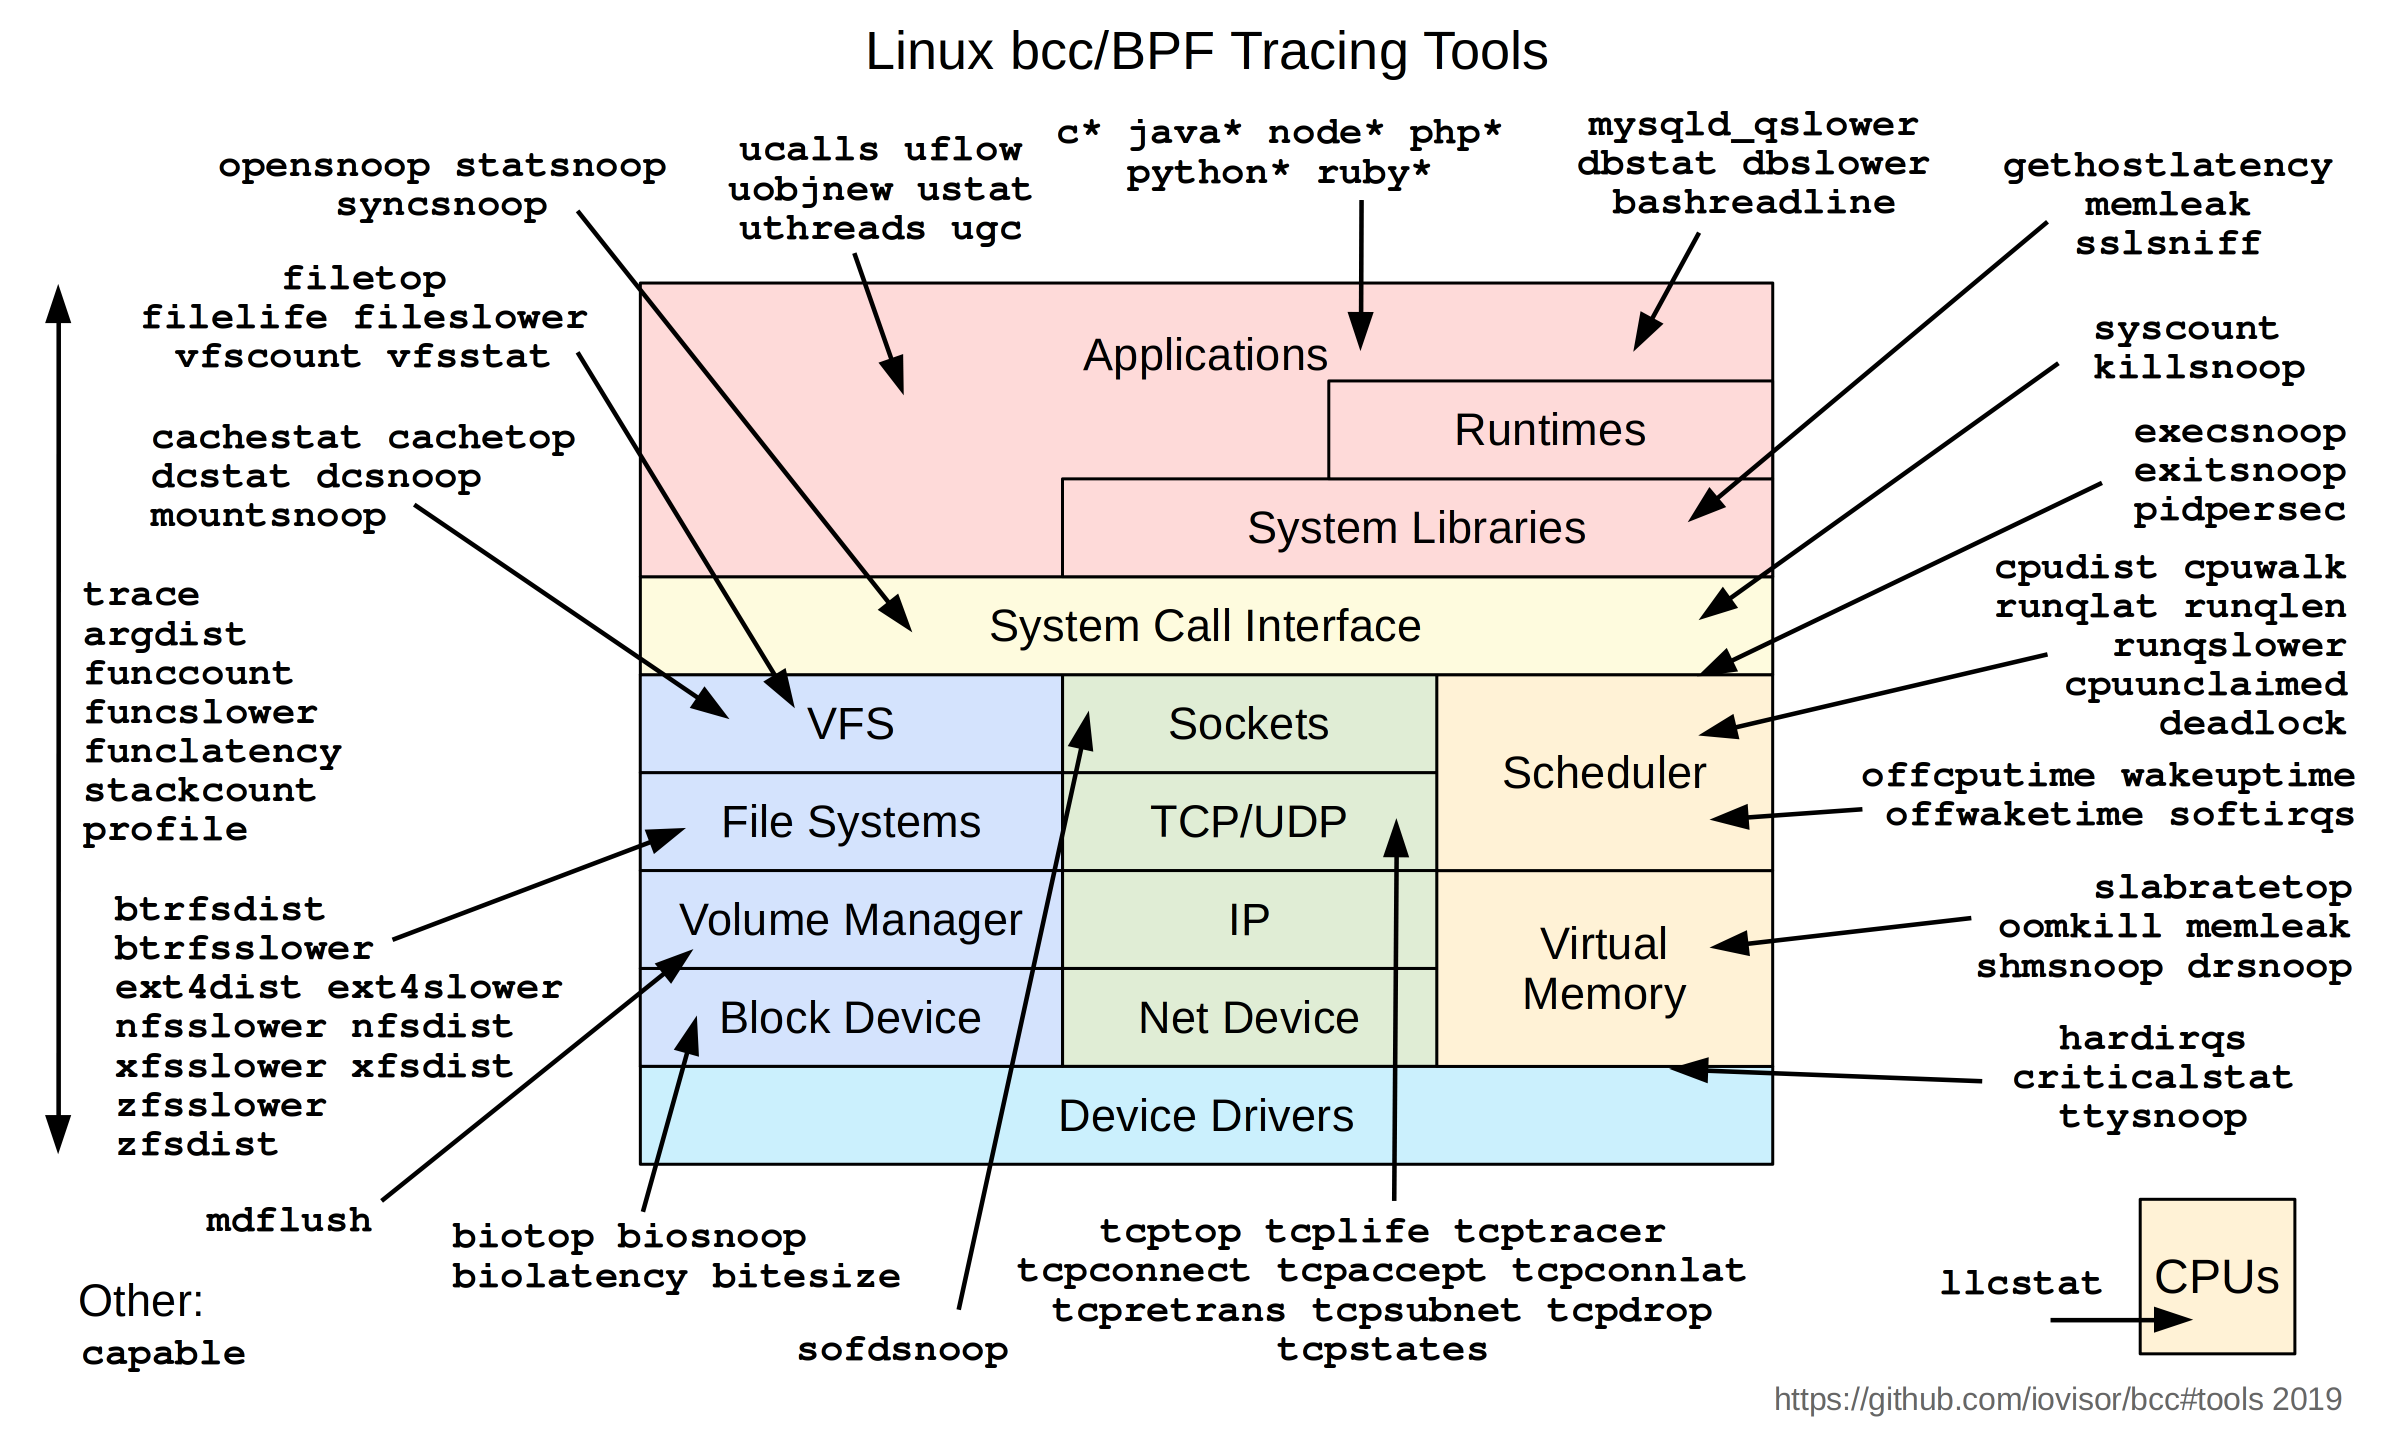
\includegraphics[scale=0.2]{bcc}
	\caption{}
	\label{image:anal:mon:bcc}
\end{figure}
It's a state-of-the-art monitoring tools bundle used by large companies (e.g. Netflix, Facebook) \cite{blog:bcc}. BCC serves as front-end (CLI) program to various eBPF-based tools. Concretely, \textit{execsnoop}, \textit{opensnoop}, \textit{tcpaccept}, \textit{tcpconnect} and \textit{tcptracer} are programs tracing \texttt{exec} syscalls, \texttt{open} syscalls, tcp \texttt{accept} and \texttt{connect} syscalls and tcp connection sessions respectively.

Some BCC tools have a mount namespace option to filter the monitored events. This can potentially select a specific container. The mount namespace is passed via a BPF map object created by the \textit{bpftool} tool \cite{git:bcc:mntns}.

\subsubsection*{monks}
\textit{Monks}\footnote{\url{https://github.com/alexandernst/monks}} works as a kernel module hijacking system calls on the target system. "Monks is like strace, but tracing all and every single process from any user, at any level" \cite{git:monks}.

\subsubsection*{execmon}
\textit{Execmon}\footnote{\url{https://github.com/kfiros/execmon}} is a similar utility intercepting the \texttt{execve} system calls in kernel-space and notifies the user. It's a kernel module combined with a user-space utility receiving events.

\subsubsection*{fswatch}
For file system monitoring there is a CLI program \textit{fswatch} \footnote{\url{https://github.com/emcrisostomo/fswatch}} acting as the API to the \textit{libfswatch}, which is ultimately an API to \textit{inotify}. It provides real time FS monitoring with a second accuracy. Fswatch distinguishes events based on the action (e.g. created, renamed, removed, owner changed).